Usein ollaan kiinnostuneita siitä, millainen yhteys on kahden asian välillä. Funktio on matemaattinen työkalu näiden yhteyksien tarkastelemiseen.

\begin{comment}
\laatikko[Funktio]{
	\termi{funktio}{Funktio} $f$ on sääntö, joka liittää jokaiseen \termi{muuttuja}{muuttujaan} $x$ täsmälleen yhden arvon $f(x)$.

	Funktiolla on \termi{määrittelyjoukko}{määrittelyjoukko} $A$, johon muuttuja $x$ kuuluu,
	ja \termi{maalijoukko}{maalijoukko} $B$, johon funktion arvot $f(x)$ kuuluvat. Merkintä
	$f\colon A \to B$ tarkoittaa, että funktion $f$ määrittelyjoukko on $A$ ja maalijoukko
	on $B$.
}
%Muokannut Jaakko Viertiö 14.12.2013
%sanoisin että funktio ei liitä muuttujiin x arvoa f(x) vaan muuttuja x on symboli joka viittaa määrittelyjoukon alkioihin. Siis p.o. Funktio f liittää jokaisen määrittelyjoukon alkioon x maalijoukon jonkin maalijoukon alkion f(x). -Jouni Kärkkäinen 9.2.2014

\end{comment}

\laatikko[Funktio]{
  \termi{funktio}{Funktio} eli \termi{kuvaus}{kuvaus} $f$ joukosta $A$ joukkoon $B$ liittää jokaiseen joukon $A$ alkioon täsmälleen yhden joukon $B$ alkion. Funktion $f$ alkioon $x$ liittämää arvoa merkitään $f(x)$.
  }  
Joukkoa $A$ sanotaan tässä $f$:n \termi{määrittelyjoukko}{määrittelyjoukoksi} ja joukkoa $B$ puolestaan $f$:n \termi{maalijoukko}{maalijoukoksi}. Tällöin voidaan merkitä lyhyesti $f\colon A \to B$. Funktion $f$ \termi{arvojoukko}{arvojoukon} muodostavat $f$:n kaikki maalijoukkoon $B$ kuuluvat arvot $f(x)$.

%Funktion käsitettä voi verrata esimerkiksi kassakoneen toimintaan. Funktioksi voidaan ajatella kassakone. Kun siihen luetaan sisään viivakoodi, antaa kassakone ulos hinnan.

\begin{esimerkki}
	Hyödykkeen ja siitä maksettavan arvonlisäveron välistä yhteyttä voidaan kuvata funktiolla. Valitaan funktion määrittelyjoukoksi tiettyjen hyödykkeiden joukko
		\[ A = \{\text{ahvenfilee}, \text{AIV-rehu}, \text{auto}, \text{runokirja},
		\text{ravintola-ateria}, \text{särkylääke}, \text{televisio}\}, \]
	ja arvojoukoksi reaaliluvut. Merkitään tätä funktiota kirjaimella $f$, jolloin
	$f\colon A \to \mathbb{R}$.
	Funktio voi liittää kuhunkin hyödykkeeseen esimerkiksi siitä maksettavan arvonlisäveroprosentin:
	$f(\text{särkylääke}) = 10$ ja $f(\text{televisio}) = 24$.

	\begin{center}
		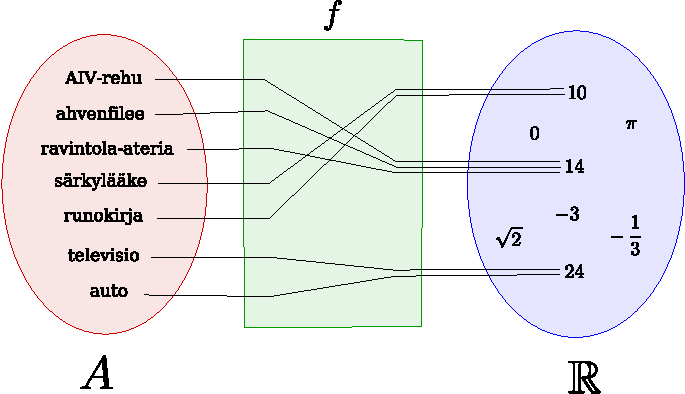
\includegraphics[width=11.5cm]{pictures/funktiokone.pdf}
	\end{center}
\end{esimerkki}

\begin{esimerkki}
Seuraavaan taulukkoon on koottu kuukausittaiset keskilämpötilat Sodankylässä vuonna 2012.

	\begin{tabular}{|c|c|c|c|c|c|c|c|c|c|c|c|}
	\hline
	tam & hel & maa & huh & tou & kes & hei & elo & syys & loka & mar & jou\\
	\hline
	$-12$ & $-16$ & $-6$ & $-3$ & $6$ & $11$ & $13$ & $12$ & $7$ & $0$ & $-4$ & $-15$\\
	\hline
	\end{tabular}
%	\caption*{Lähde: Ilmatieteen laitos}

Taulukon perusteella voidaan määritellä funktio $f$, joka kuvaa kuukaudet keskilämpötiloiksi. Määrittelyjoukko ovat vuoden kaikki kuukaudet, maalijoukkoon kuuluvat kaikki mahdolliset lämpötilat, ja arvojoukko koostuu funktion kaikista arvoista, siis eri kuukausien keskilämpötiloista. Nyt esimerkiksi $f(\text{tam}) = -12$ ja $f(\text{tou}) = 6$.

%TÄHÄN VOISI LAITTAA KUVAN KUVAAJASTA
\end{esimerkki}

\begin{esimerkki}
Seuraava kuva esittää erään suotuisissa oloissa kehittyvän bakteerikannan massaa ajan $t$ funktiona $m$.

\begin{kuva}
    kuvaaja.pohja(0, 8, 0, 8)
    kuvaaja.piirra("1.4**x", nimi = "$y=m(t)$")
\end{kuva}

Alkutilanteessa eli ajanhetkellä $t=0$ bakteerikannan massa $m(t)$ on $m(0)=1$ gramma. Kahden tunnin kuluttua bakteerikannan massa on $m(2)\approx 2,0$ grammaa ja kuuden tunnin kuluttua vastaavasti $m(6)\approx 7,5$ grammaa. 
\end{esimerkki}

Funktioiden merkitsemiseen liittyy joitakin vakiintuneita tapoja:
\begin{description}
	\item[1)] Merkintä $f(x) = y$ luetaan esimerkiksi: ''funktio $f$ saa arvon $y$ pisteessä $x$'' tai lyhyemmin: ''$f$ arvolla $x$ on $y$.''
	\item[2)] Funktion määrittely- ja maalijoukot jätetään usein merkitsemättä, jos ne voidaan päätellä asiayhteydestä.
		Tällä kurssilla funktiot ovat yleensä reaaliluvuilta reaaliluvuille.
	\item[3)] Usein kirjoitetaan esimerkiksi ''funktio $f(x) = x^2+3x$'', vaikka tarkkaan ottaen funktio on $f$ ja
		$f(x)$ on sen saama arvo pisteessä $x$.
	\item[4)] Toisinaan funktiolle ja funktion kuvaajalle ei tehdä selkeää eroa:
		$y = f(x)$ samaistetaan koordinaatistoon piirretyn funktion kuvaajan kanssa.
		Oikeastaan funktio ja sen kuvaaja ovat kuitenkin eri asioita.
	\item[5)] Niitä x:n arvoja, joilla funktio saa arvon 0, sanotaan funktion \termi{nollakohta}{nollakohdiksi}.
\end{description}

Huomaa seuraavien käsitteiden erot:
\laatikko[Käsitteitä]{
Määritellään funktio $f$ seuraavasti: $f(x)=3x-2$
	\luettelo{
		§ $f$ on funktion nimi
		§ merkintä $f(x)$ tarkoittaa funktion $f$ \textit{arvoa kohdassa $x$}
		§ $3x-2$ on \textit{lauseke}, jolla $f(x)$ on määritelty
		§ \textit{Yhtälö} $f(x)=3x-2$ kertoo, että funktion $f$ arvo kohdassa $x$ on yhtäsuuri lausekkeen $3x-2$ kanssa
		§ $x$ on funktion muuttuja
	}
}

\subsection*{Reaalifunktiot}

Funktioita, jotka määritellään reaaliluvuilla, ja jotka saavat arvokseen reaalilukuja, kutsutaan reaalifunktioiksi.
Funktiolla, erityisesti reaalifunktioilla, on usein jokin selkeä sääntö, joka voidaan kirjoittaa matemaattisena lausekkeena.

\begin{esimerkki}
Jos neliön sivun pituutta merkitään muuttujalla $x$, voidaan pinta-alaa kuvata funktiolla $A\colon A(x) = x^2$.
\end{esimerkki} 

Reaalifunktioita voidaan havainnollistaa koordinaatistossa \textit{kuvaajien} avulla. Funktion $f$ kuvaajassa koordinaatistoon piirretään ne pisteet $(x, y)$, joiden $y$-koordinaatti on $f$:n arvo $x$-koordinaatissa. Reaalifunktioilla ei kuitenkaan voida laskea $y = f(x)$ kaikilla $f$:n määrittelyjoukon luvuilla $x$, joten esimerkiksi graafiset laskimet laskevat $y = f(x)$ ''riittävän monella'' luvulla ja sovittavat kuvaajan niiden perusteella. Funktioiden kuvaajia voi piirtää helposti paitsi graafisilla laskimilla, myös tietokoneohjelmilla sekä esimerkiksi verkossa Wolfram Alphalla (\url{http://www.wolframalpha.com/}). 

% Tarvitaan kuvien ja taulukkojen vierekkäin laittamiseen.
\def\vcent#1{\mathsurround0pt$\vcenter{\hbox{#1}}$}

\begin{luoKuva}{suoraesim}
    kuvaaja.pohja(-4, 4, -3, 2, korkeus = 4, nimiX = "$x$", nimiY = "$y$")
    with vari("red"): kuvaaja.piirra(lambda x: 0.5 * x - 1, kohta = 3, suunta = 135, nimi = "$y = f(x)$")
    piste((-3, -2.5))
    piste((-2, -2))
    piste((-1, -1.5))
    piste((0, -1))
    piste((1, -0.5))
    piste((2, 0))
    piste((3, 0.5))
\end{luoKuva}
\begin{esimerkki}
	Funktion $f \colon f(x) = \frac{x}{2} - 1$ kuvaaja sisältää kaikki pisteet $(x, y)$, joilla pätee $y = \frac{x}{2} - 1$. Funktion kuvaaja leikkaa x akselin kun x = 2, tämä pistettä sanotaan funktion nollakohdaksi. (Huomaa, että funktioilla voi olla myös useampia nollakohtia, tai ei yhtään nollakohtaa.)
	\begin{center}
		\begin{tabular}{cc}
			\begin{tabular}{|r|l|}
				\hline
				$x$ & $y = f(x)$ \\
				\hline
				$-3$ & $-2,5$ \\
				$-2$ & $-2$ \\
				$-1$ & $-1,5$ \\
				$0$ & $-1$ \\
				$1$ & $-0,5$ \\
				$2$ & $0$ \\
				$3$ & $0,5$ \\
				\hline
			\end{tabular} &
			\vcent{\naytaKuva{suoraesim}}
		\end{tabular}
	\end{center}
\end{esimerkki}

\begin{luoKuva}{paraabeli}
    kuvaaja.pohja(-3, 3, -1, 6, korkeus = 5, nimiX = "$x$", nimiY = "$y$")
    with vari("red"): kuvaaja.piirra(lambda x: x * x, kohta = 1.5, nimi = "$y = f(x)$")
    piste((-2, 4))
    piste((-1, 1))
    piste((-0.5, 0.25))
    piste((0, -0))
    piste((0.5, 0.25))
    piste((1, 1))
    piste((2, 4))
\end{luoKuva}
\begin{esimerkki}
	Funktion $f(x) = x^2$ kuvaaja sisältää kaikki pisteet $(x, y)$, joilla pätee $y = x^2$. Kuvaajan nollakohta on tässä tapauksessa, kun $x$ saa arvon 0, koska $y = 0^2 = 0$.
	\begin{center}
		\begin{tabular}{cc}
			\begin{tabular}{|r|l|}
				\hline
				$x$ & $y = f(x)$ \\
				\hline
				$-2$ & $4$ \\
				$-1$ & $1$ \\
				$-0,5$ & $0.25$ \\
				$0$ & $0$ \\
				$0,5$ & $0.25$ \\
				$1$ & $1$ \\
				$2$ & $4$ \\
				\hline
			\end{tabular} &
			\vcent{\naytaKuva{paraabeli}}
		\end{tabular}
	\end{center}
\end{esimerkki}

\begin{luoKuva}{deg3polynomiesim}
    kuvaaja.pohja(-3, 3, -4, 9, korkeus = 6, leveys = 7, nimiX = "$x$", nimiY = "$y$")
    with vari("red"): kuvaaja.piirra(lambda x: x**3 - 5 * x + 2, kohta = 2.2, nimi = "$y = f(x)$")
    piste((-1-sqrt(2), 0))
    piste((sqrt(2)-1, 0))
    piste((2, 0))
\end{luoKuva}
\begin{esimerkki}
	Funktion $f(x) = x^3-5x+2$ kuvaaja sisältää kaikki pisteet $(x, y)$, joilla pätee $y = x^3-5x+2$. Funktiolla on tässä tapauksessa kolme nollakohtaa:
	\begin{center}
	\naytaKuva{deg3polynomiesim}
	\end{center}
\end{esimerkki}

\subsection*{Määrittelyjoukko ja arvojoukko}

%Funktion määrittelyjoukko koostuu niistä muuttujan arvoista, joilla funktio on määritelty, eli joilla funktion arvo voidaan laskea.

Funktion \termi{määrittelyjoukko}{määrittelyjoukko} on niiden arvojen joukko, joille funktion arvo on olemassa. Jos määrittelyjoukkoa ei ole mainittu erikseen, määrittelyjoukon tarkoitetaan tavallisesti olevan \textit{mahdollisimman laaja reaalilukujen osajoukko} johon kuuluville arvoille funktion arvon voi laskea. %Jouni Kärkkäinen 92.2.2014

\begin{esimerkki}
	 Määritellään funktio $g$ lausekkeella \[ g(x) = \sqrt{x}. \]
	 Mikä on funktion $g$ määrittelyjoukko?
	 \begin{esimratk}
		Neliöjuuri $\sqrt{x}$ on määritelty, kun $x\geq{0}$. Funktion $g$ määrittelyehto on siis $x\geq{0}$ ja määrittelyjoukko koostuu nollasta ja sitä suuremmista reaaliluvuista.
	 \end{esimratk}
	 \begin{esimvast}
	  $x\geq{0}$.
	 \end{esimvast}
\end{esimerkki}
%Lisännyt Jaakko Viertiö 14.12.2013

Käytännössä määrittelyjoukon rajoituksia tarvitaan yllä esitetyn parillisen juuren lisäksi esimerkiksi silloin kun funktiossa esiintyy muuttuja nimittäjässä. Tällöin on huomioitava, ettei nimittäjässä saa olla nollaa millään muuttujan $x$ arvolla. Soveltavissa tehtävissä saatetaan myös rajoittaa määrittelyjoukkoa vaikkapa siksi, että pituus ei voi olla negatiivinen.

\begin{esimerkki}
	Määritellään funktio $f$ lausekkeella \[ f(x) = \frac{1}{x-1}. \]
	Mikä on funktion määrittelyjoukko?
	\begin{esimratk}
	Funktio $f$ on määritelty, kun nimittäjä $x-1$ on erisuuri kuin $0$. Tämä toteutuu kaikilla $x$:n arvoilla lukuun ottamatta arvoa $x = 1$. Funktion määrittelyjoukkoon kuuluvat siis kaikki reaaliluvut paitsi luku $1$.
	\end{esimratk}
	\begin{esimvast}
		Funktion $f$ määrittelyjoukko on reaalilukujen joukko poislukien luku $1$.
	\end{esimvast}
\end{esimerkki}


Funktion \termi{arvojoukko}{arvojoukko} sisältää täsmälleen ne maalijoukon alkiot,
jotka funktio saa arvokseen ainakin yhdessä pisteessä.

\begin{esimerkki}
	Mikä on edellä määritellyn funktion $f$ arvojoukko?
	% korjaa
	\begin{esimratk}
		Arvojoukon selvittämiseksi tutkitaan, millä luvun $a$ arvoilla
		yhtälöllä $f(x) = a$ on ratkaisu. Oletetaan, että $x \neq 1$ (ks. edellinen esimerkki).
		\begin{align*}
			a &= \frac{1}{x-1} & &| \, \cdot (x-1), \; \text{sillä} \; x \neq 1 \\
			a(x-1) &= 1
		\end{align*}
		Havaitaan, että jos $a = 0$, yhtälöllä ei voi olla ratkaisua, koska $0 \cdot (x-1) = 0 \neq 1$.
		Oletetaan jatkossa, että $a \neq 0$.
		\begin{align*}
			a(x-1) &= 1 & &| \, : a, \; \text{sillä} \; a \neq 0 \\
			x-1 &= \frac{1}{a} \\
			x &= 1+\frac{1}{a}
		\end{align*}
		Havaitaan, että yhtälöllä on ratkaisu kaikilla $a \neq 0$.
	\end{esimratk}
	\begin{esimvast}
		Funktion $f$ arvojoukko on reaalilukujen joukko poislukien luku $0$.
	\end{esimvast}
\end{esimerkki}
%Kuva tähän esimerkkiin? Näkisi miten lähtö- ja arvojoukkojen "puuttuvat" alkiot näkyvät kuvaajassa.

\begin{esimerkki}
	Tarkastellaan reaalifunktiota $f(x)=x^2$. Funktion $f$ \textit{määrittelyjoukko} on selkeästi koko reaalilukujen joukko, sillä toinen potenssi $x^2$ on määritelty, olipa muuttuja $x$ mikä reaaliluku tahansa. Funktio $f$ on reaalifunktio, joten sen arvot ovat reaalilukuja. Sen \textit{maalijoukko} on siis koko reaalilukujen joukko. Kuitenkin, koska parillisena potenssina $x^{2}\geq0$, olipa $x$ mikä luku hyvänsä, funktion $f$ \textit{arvojoukko} on kaikki positiiviset reaaliluvut.
	
\begin{center}
\begin{kuva}
	kuvaaja.pohja(-5, 5, -2, 8, korkeus=7, nimiX = "$x$", nimiY = "$y$")
	with vari("red"): kuvaaja.piirra(lambda x: x**2, kohta=2.5, nimi="$y=x^2$")
\end{kuva}
\end{center}
	
	
\end{esimerkki}
	
\subsection*{Paloittain määritelty funktio}

Kappaleessa \ref{neliojuuri} sivuttiin itseisarvon määritelmää. Itseisarvofunktio $f: f(x) = \lvert x \rvert$ voidaan määritellä seuraavasti. \\ 
$$
f\colon \mathbb{R} \to \mathbb{R_+}, \\ \lvert x \rvert = \begin{cases}
                 x & \text{jos } x \geq 0 \\
                 -x & \text{jos } x < 0
              
                \end{cases}
$$

Funktio siis jättää ei-negatiiviset luvut ennalleen, mutta vaihtaa negatiivisen luvun vastaluvukseen, ja arvojoukko koostuu pelkästään ei-negatiivisista luvuista. Funktio on määritelty kahdessa eri osassa: lähtöjoukon alkion arvosta riippuen valitaan sille sovellettava lauseke.

\begin{esimerkki}
 
 Määritellään funktio $g\colon \mathbb{R} \to \mathbb{R}$ lausekkeilla
 $$
 g(x) = \begin{cases}
         \frac{x}{x} & \text{jos } x \neq 0 \\
         1 & \text{jos } x = 0
        \end{cases}
$$
 
Mikä on funktion arvojoukko? Miksi määrittelemme kohdan $x = 0$ erikseen?

\begin{esimratk}
Kun $x \neq 0$, osamäärästä $\frac{x}{x}$ saadaan aina $1$. Kohdassa $x=0$ funktion arvoksi on puolestaan määritelty $1$. Näin ollen funktion $g$ arvojoukko koostuu yhdestä ainoasta luvusta, ykkösestä. Koska lauseke $\frac{0}{0}$ ei ole määritelty, määrittelemme kohdan $x=0$ erikseen. Funktio on siis vakioarvoinen ja voisimme kirjoittaa sen yksinkertaisesti $g\colon g(x) = 1$. 

\end{esimratk}
\end{esimerkki}